% Derived from week_1 tabular-classification-report/assets/report_template.tex:
% ACM sigconf double columns, booktabs, graphicx, xeCJK, Windows CJK fonts,
% and introduction/data/method/results/discussion/conclusion structure.
% Self-contained source: title, abstract, and content are included below.
% XeLaTeX: compile until cross-references stabilize (normally three passes).
\documentclass[sigconf,balance=false]{acmart}
\usepackage{booktabs}
\usepackage{graphicx}
\usepackage{float}
\usepackage{xeCJK}
\setCJKmainfont{SimSun}[BoldFont=SimHei,ItalicFont=KaiTi,AutoFakeBold=2]
\setCJKsansfont{SimHei}[BoldFont=SimHei,AutoFakeBold=2]
\setCJKmonofont{SimSun}
\AtBeginDocument{\setlength{\parindent}{2em}}
\setcopyright{none}
\settopmatter{printacmref=false}
\renewcommand\footnotetextcopyrightpermission[1]{}
\fancypagestyle{plain}{\fancyhf{}\fancyfoot[C]{\thepage}\renewcommand{\headrulewidth}{0pt}}
\begin{document}
\title{冻结视觉骨干与 SE 门控的物种分类实验}
\author{实验项目技术报告}
\begin{abstract}
本报告记录两种冻结视觉骨干及其分类头前 SE 门控的配对实验。100 类、1000 张图像按 600/200/200 划分，两个骨干使用相同测试样本。ResNet-50 基线及 SE 的 Top-1 准确率分别为 45.00\% 和 51.50\%；ViT-B/16 分别为 35.00\% 和 34.50\%。结果属于单种子、小样本实验。
\end{abstract}
\maketitle
\pagestyle{plain}
\suppressfloats[t]


\section{引言}
本实验比较 ImageNet 预训练的 ResNet-50 与 ViT-B/16 冻结表征在物种分类中的表现，并在分类头前加入 SE 门控作配对消融。实际运行入口为 \path{scripts/run_task1.py} 和 \path{scripts/run_task2.py}；完整配置与结果分别保存在 \path{results/task1/} 和 \path{results/task2/}。

\section{数据集}
本地 Parquet 共 1000 张、100 类，每类 10 张，仅以图像及标签建模。固定种子 42，按类划分训练、验证、测试集各 6、2、2 张，总数分别为 600、200、200；实际索引与 ID 见 \path{results/task1/split.json}。测试集为本地保留子集，并非官方测试集。图片转 RGB 后按对应权重的预处理缩放、中心裁剪至 $224\times224$ 并标准化。

\section{方法与实验设置}
两模型使用 torchvision 的 ResNet50\_Weights.IMAGENET1K\_V2 和 ViT\_B\_16\_Weights.IMAGENET1K\_V1；不同预训练配方限制了单独归因于架构的解释。冻结骨干并分别对 ResNet layer4 空间特征及 ViT 最终图像块 token（排除 CLS）求均值，维度为 2048 和 768。标准化参数仅由训练特征估计。实验复用了旧实验的同方式特征，并重新训练基线分类头；迁移记录见 \path{results/task1/feature_migration.json}。

分类头为带偏置的线性层；SE 组在标准化特征和头之间加入降维比例 16 的两层门控。每对使用相同特征、划分、分类头初始参数和优化设置。CPU 上以 AdamW、学习率 0.01、权重衰减 0.01，全批次训练 300 轮，按验证交叉熵最低选择模型。种子、环境与完整配置分别见两项任务的 \path{config.json}。

\section{实测结果}
表~\ref{tab:vision} 为同一 200 张测试图片上的结果；Top-1、Top-5 和 Macro-F1 均以百分数表示，Macro-F1 对 100 类等权平均。来源为 \path{results/task2/comparison.csv}，其中基线引用 Task 1 指标，数值四舍五入到两位小数。
\begin{table}[H]
\caption{冻结骨干与 SE 配对测试结果（\%）。}\label{tab:vision}
\centering\small
\begin{tabular}{lrrr}\toprule
模型 & Top-1 & Top-5 & Macro-F1 \\
\midrule
ResNet-50 & 45.00 & 72.00 & 41.25 \\
ResNet-50 + SE & 51.50 & 71.50 & 46.76 \\
ViT-B/16 & 35.00 & 64.00 & 31.61 \\
ViT-B/16 + SE & 34.50 & 60.50 & 30.13 \\
\bottomrule\end{tabular}
\end{table}

图~\ref{fig:loss} 是由四组保存的训练记录绘制的完整 300 轮曲线；验证损失最低的轮次用于选模。原图见 \path{results/figures/loss_curves_full.png}，原始记录见各模型目录的 \path{history.json}。



\begin{figure}[htbp]
\centering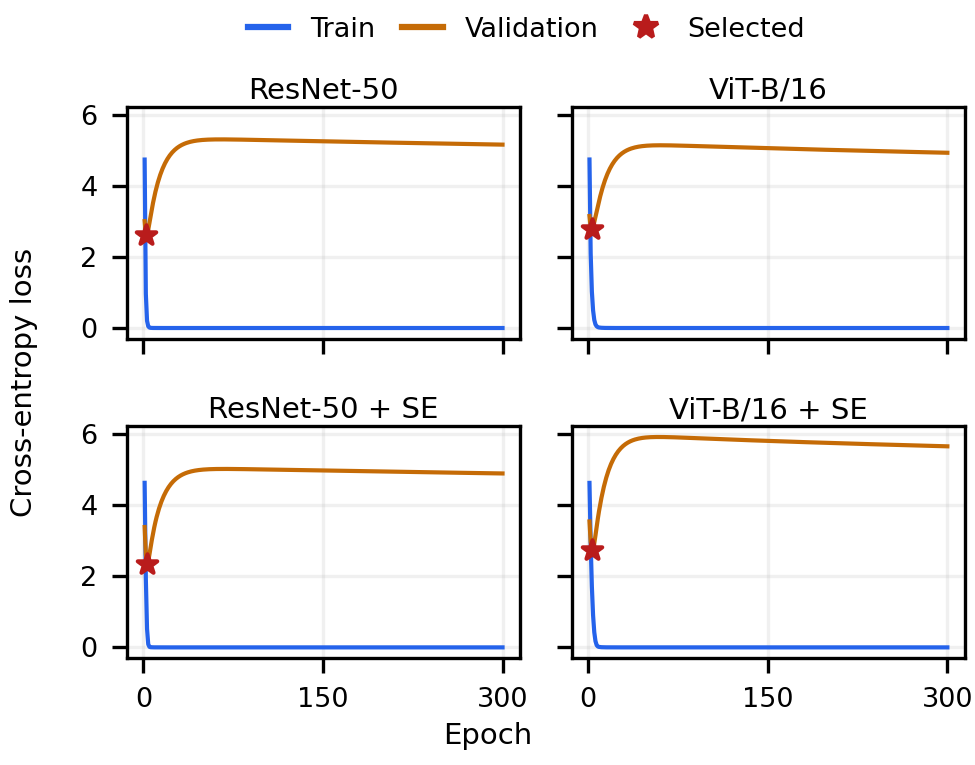
\includegraphics[width=\linewidth]{figures/loss_curves_column.png}
\caption{四组模型的训练与验证损失，标记为验证损失最低轮次。}\label{fig:loss}
\end{figure}
\section{讨论}
本次加入 SE 后 ResNet 的 Top-1 提高 6.50 个百分点，ViT 下降 0.50 个百分点；这只描述当前配对结果。验证损失在早期达到最低，之后上升，提示分类头存在过拟合。每类测试仅两张，且单种子划分未按拍摄者或重复图像分组，不能据此推断独立来源泛化或普遍的架构优势。逐样本复核记录见 \path{results/task1/verification.txt} 与 \path{results/task2/verification.txt}。
\section{结论}
当前记录中 ResNet-50 + SE 的测试 Top-1 最高，而 SE 对 ViT 未带来提升；多种子或独立测试集仍需后续实验验证。
\end{document}
